\documentclass{article}

\usepackage[a4paper, margin=1in]{geometry}

% For positioning figures (eg. images) with [H]
\usepackage{float}

% Used for \SI and SI units
\usepackage[
  separate-uncertainty=true,
  multi-part-units=single
]{siunitx}
\newcommand{\unc}[2]{\(\pm\SI{#1}{#2}\)}
\newcommand{\punc}[2]{\(\pm\SI{#1}{\percent}\) \si{#2}}

% Fancy tables innit
% https://tablesgenerator.com/latex_tables
\usepackage{booktabs}
\usepackage{tabularx}

% For \abs
\usepackage{mathtools}
\DeclarePairedDelimiter\abs{\lvert}{\rvert}%

% Swap the definition of \abs* so that it resizes the size of the
% brackets, and the starred version does not.
\makeatletter
\let\oldabs\abs
\def\abs{\@ifstar{\oldabs}{\oldabs*}}
\makeatother

% For including graphs via \includegraphics
\usepackage{graphicx}
\graphicspath{{assets}}

% Graph shortcuts
\newcommand{\graph}[2]{
  \begin{figure}[H]
    \medskip
    \centering
    \includegraphics[width=1\linewidth]{#1}
    \caption{#2}\label{fig:#1}
  \end{figure}
}

% Links
\usepackage{hyperref}
\hypersetup{colorlinks=true, linkcolor=blue, urlcolor=cyan, citecolor=blue}
\urlstyle{same}

% show TODO's in red
\newcommand{\todo}[1]{{\color{red}{\footnotesize[TODO:\@ #1]}}}
% to remove all todo's
%\newcommand\todo[1]{}

\author{Luis F.}
\title{Wire Resistance Lab}

\begin{document}

\maketitle

\section{Lab Design}
\subsection{Research Question}

\begin{itemize}
  \item Research question: How is the resistance of a wire dependent on its cross-sectional area?
  \item Independent variable: Cross-sectional area of the wire
  \item Dependent variable: Resistance of the wire
\end{itemize}

The hypothesis is that the resistance of a wire is inversely proportional to its cross-sectional area. This can be seen in equation~\ref{eq:resistance}, the equation for resistance. As the cross-sectional area \(A\) increases, the resistance \(R\) decreases.

\begin{equation}\label{eq:resistance}
  R = \frac{\rho L}{A}
\end{equation}

\subsection{Controlled Variables}

The dependent variable, resistance, will be measured using a multimeter. The probes used to measure the resistance and their position on the wire will be kept constant.

The length of the wire between the probes will also be kept constant, at \SI{40\pm0.5}{\centi\metre}, as can be seen in figure~\ref{fig:lab-setup}. This uncertainty was chosen as the wire was measured using the ruler on the wire board, and while the smallest division was \SI{1}{\milli\metre}, the wire was slightly elevated above the ruler, making it difficult to measure accurately due to parallax errors. Therefore we decided that \unc{0.5}{\centi\metre} was a reasonable uncertainty.

The temperature of the wire will be kept constant by taking the measurements in a room with a constant temperature, controlled by thermostat, and performing the resistance readings quickly to avoid any significant temperature changes. Furthermore, we waited between trials to ensure the wire had cooled down to room temperature, using this time to record the data from the previous trial.

\begin{figure}[H]
  \medskip
  \centering
  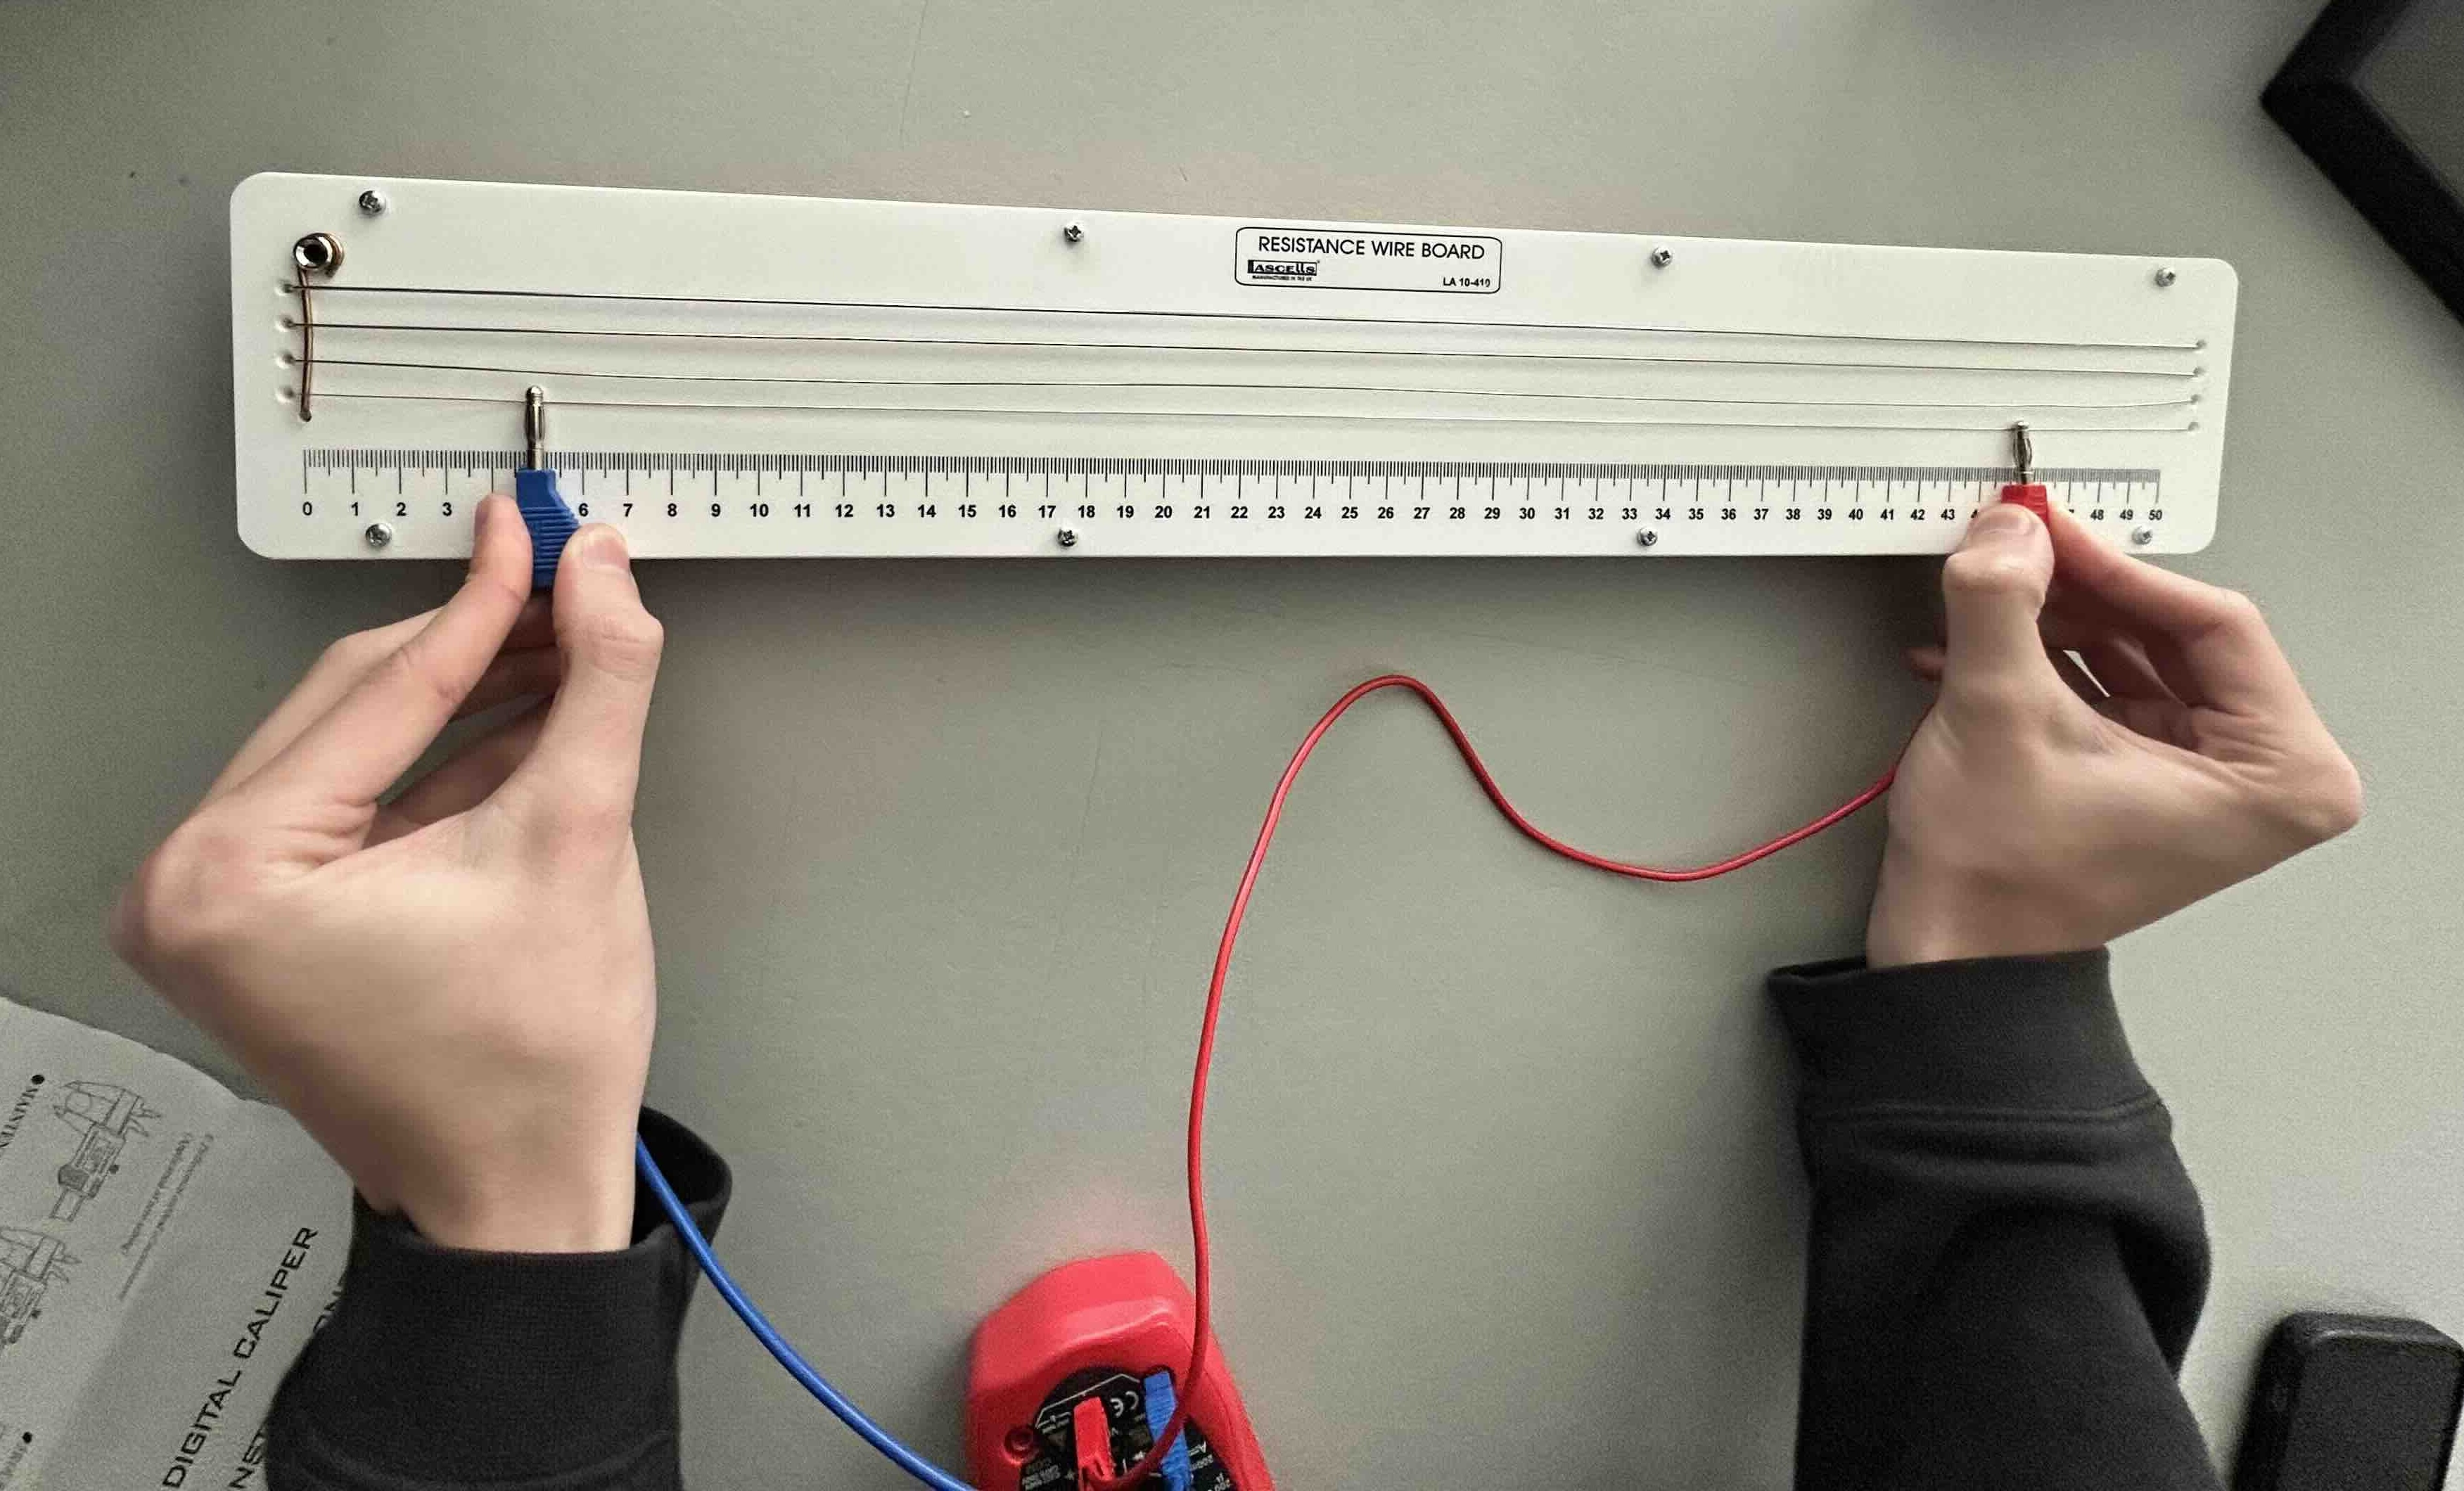
\includegraphics[width=1\linewidth]{lab-setup}
  \caption{Lab setup, where constant variables can be observed}\label{fig:lab-setup}
\end{figure}

\subsection{Independent Variable}

The independent variable is the cross-sectional area of the wire. The cross-sectional area will be varied by using wires of different diameters. The diameters of the wires used can be seen in table~\ref{tab:given-data}. The cross-sectional area \(A\)
% Feedback: Just say A, that is the variable given in the equation.
% - Instead of CSA, use \(A\)
of the wire can be calculated using equation~\ref{eq:csa}, the formula for the area of a circle, where \(r\) is the radius of the wire. The radius of the wire is half of the diameter, so the formula can be rewritten in terms of the diameter \(d\).

\begin{equation}\label{eq:csa}
  A = \pi r^2 = \frac{\pi d^2}{4}
\end{equation}

An uncertainty of \punc{1}{\milli\metre} will be used for wire diameter, and \punc{1}{\ohm\metre} for resistivity, as they were given values with no stated uncertainty, and 1\% is the standard default uncertainty we were instructed to use by our teacher. The uncertainty for \(A\) can be derived using the formula for propagating powers in uncertainties, which results in an uncertainty of \punc{2}{\milli\metre\squared}.

\todo{Explain how the uncertainty for CSA was calculated}

\begin{table}[H]
  \centering
  \begin{tabular}{@{}ccc@{}}
    \toprule
    % Feedback: This resistivity has no unc, it is given and theoretical.
    Diameter \punc{1}{\milli\metre} & CSA \punc{2}{\milli\metre\squared} & Resistivity (\si{\ohm\metre}) \\ \midrule
    \num{1.00}                      & \num{0.79}                         & \num{1.08e-6}                 \\
    \num{0.80}                      & \num{0.50}                         & \num{1.08e-6}                 \\
    \num{0.63}                      & \num{0.31}                         & \num{1.08e-6}                 \\
    \num{0.49}                      & \num{0.19}                         & \num{1.08e-6}                 \\ \bottomrule
  \end{tabular}
  \caption{Pre-experiment given wire data}\label{tab:given-data}
\end{table}

For example, using equation~\ref{eq:csa}, the cross-sectional area \(A\) of the wire with a diameter of \SI{1.00}{\milli\metre} can be calculated as follows:

\begin{equation*}
  A = \frac{\pi \times \SI{1.00}{\milli\metre}^2}{4} = \frac{\pi}{4} \approx \SI{0.79}{\milli\metre\squared}
\end{equation*}

For this experiment, five trials were performed for each wire diameter, measuring the resistance of the wire for each trial. This will result in a total of 20 trials. 25 trials would have been preferred, however our wire board only had four different wires available.

% Feedback: Ok, good. Where is your method and apparatus?

\section{Data Collection and Processing}

\begin{table}[H]
  \centering
  \begin{tabular}{@{}cccccccc@{}}
    \toprule
    % https://tex.stackexchange.com/a/482550
    & & \multicolumn{6}{@{}c@{}}{Resistance \unc{0.1}{\ohm}} \\
    \cmidrule(l){3-8}
    Length \unc{0.5}{\centi\metre} & CSA \punc{2}{\milli\metre\squared} & T1 & T2 & T3 & T4 & T5 & Average \\ \midrule
    \num{40.0} & \num{0.79} & \num{1.2} & \num{1.0} & \num{1.2} & \num{1.6} & \num{1.0} & \num{1.20}        \\
    \num{40.0} & \num{0.50} & \num{1.9} & \num{1.7} & \num{1.6} & \num{1.5} & \num{1.6} & \num{1.66}        \\
    \num{40.0} & \num{0.31} & \num{1.8} & \num{2.9} & \num{1.8} & \num{1.7} & \num{1.7} & \num{1.98}        \\
    \num{40.0} & \num{0.19} & \num{3.9} & \num{4.5} & \num{3.9} & \num{3.8} & \num{3.6} & \num{3.94}        \\ \bottomrule
  \end{tabular}
  \caption{Raw wire data collected}\label{tab:raw-data}
\end{table}

The average resistance for each wire diameter was calculated by taking the arithmetic mean of the five trials. An example of this calculation can be seen in equation~\ref{eq:average-resistance}.

The uncertainty for the resistance was chosen to be \unc{0.1}{\ohm}, as the multimeter used went up by increments of \SI{0.1}{\ohm}, and this is the convention for digital readings.

\begin{equation}\label{eq:average-resistance}
  R_\mathrm{avg} = \frac{1.2 + 1.0 + 1.2 + 1.6 + 1.0}{5} = \SI{1.20}{\ohm}
\end{equation}

% Feedback: Ok, clear. Consider adding grid lines to your table.
% - I disagree, I think tables look cleaner without grid lines.

To calculate the uncertainty for the average resistance, we can calculate the difference from the mean for each trial, and then take the average of these differences. This is done in table~\ref{tab:diff-from-mean}.

\begin{table}[H]
  \centering
  \begin{tabular}{@{}cccccccc@{}}
    \toprule
    % https://tex.stackexchange.com/a/482550
    & & \multicolumn{6}{@{}c@{}}{Difference from mean resistance (\si{\ohm})} \\
    \cmidrule(l){3-8}
    Length \unc{0.5}{\centi\metre} & CSA \punc{2}{\milli\metre\squared} & T1 & T2 & T3 & T4 & T5 & Average \\ \midrule
    \num{40.0} & \num{0.79} & \num{0.0} & \num{0.2} & \num{0.0} & \num{0.4} & \num{0.2} & \num{0.2}         \\
    \num{40.0} & \num{0.50} & \num{0.2} & \num{0.0} & \num{0.1} & \num{0.2} & \num{0.0} & \num{0.1}         \\
    \num{40.0} & \num{0.31} & \num{0.2} & \num{0.9} & \num{0.2} & \num{0.3} & \num{0.3} & \num{0.4}         \\
    \num{40.0} & \num{0.19} & \num{0.0} & \num{0.6} & \num{0.0} & \num{0.1} & \num{0.3} & \num{0.2}         \\ \bottomrule
  \end{tabular}
  \caption{Differences from mean resistance for each wire}\label{tab:diff-from-mean}
\end{table}

\todo{Show example calcs}

Putting this together, we get table~\ref{tab:processed-data}, which shows the processed data for each trial, including the average resistance and the uncertainty for the average resistance.

\begin{table}[H]
  \centering
  \begin{tabular}{@{}cccl@{}}
    \toprule
    Length \unc{0.5}{\centi\metre} & CSA \punc{2}{\milli\metre\squared} & Average resistance & Uncertainty (\si{\ohm}) \\ \midrule
    \num{40.0}                     & \num{0.79}                         & \num{1.20}         & \num{\pm0.2}            \\
    \num{40.0}                     & \num{0.50}                         & \num{1.66}         & \num{\pm0.1}            \\
    \num{40.0}                     & \num{0.31}                         & \num{1.98}         & \num{\pm0.4}            \\
    \num{40.0}                     & \num{0.19}                         & \num{3.94}         & \num{\pm0.2}            \\ \bottomrule
  \end{tabular}
  \caption{Processed wire trials}\label{tab:processed-data}
\end{table}

% Feedback: No need to put units in the data, put them in the header
% - (for uncertainty column, done)

% Feedback: Why is the unc for .31 so much bigger?

% Feedback: You should have your L and A in m and metres squared.
% - Done in table~\ref{tab:processed-data-normalised}. I initially had this done but commented it out, as I thought it was unnecessary. I have now uncommented it. Where in the rubric does it say to normalise the data?

Normalising the units of length into metres and CSA into metres squared gives us table~\ref{tab:processed-data-normalised}.

\begin{table}[H]
  \centering
  \begin{tabular}{@{}cccl@{}}
    \toprule
    Length \unc{0.005}{\metre} & CSA \punc{2}{\metre\squared} & Average resistance & Uncertainty (\si{\ohm}) \\ \midrule
    \num{0.400}                & \num{7.9e-7}                 & \num{1.20}         & \num{\pm0.2}            \\
    \num{0.400}                & \num{5.0e-7}                 & \num{1.66}         & \num{\pm0.1}            \\
    \num{0.400}                & \num{3.1e-7}                 & \num{1.98}         & \num{\pm0.4}            \\
    \num{0.400}                & \num{1.9e-7}                 & \num{3.94}         & \num{\pm0.2}            \\ \bottomrule
  \end{tabular}
  \caption{Processed and normalised wire trials}\label{tab:processed-data-normalised}
\end{table}

Having this, we can construct figure~\ref{fig:resistance-vs-csa}, a graph of our independent variable, cross-sectional area, against our dependent variable, resistance. However, the graph will be using the unnormalised data from table~\ref{tab:processed-data} as Excel is not accurate enough to process numbers as small as the ones in table~\ref{tab:processed-data-normalised}, and produces inaccurate trendlines.

\graph{resistance-vs-csa}{Resistance vs cross-sectional area}

The relationship between CSA and resistance appears to be approximately inversely proportional, as seen in the line of best fit shown in equation~\ref{eq:best-fit} and the approximate relationship in equation~\ref{eq:approximate-fit}.

\begin{equation}\label{eq:best-fit}
  R = 0.9438 \times A^{-0.79}
\end{equation}

\begin{equation}\label{eq:approximate-fit}
  R \propto A^{-0.79} \approx R \propto A^{-1} \implies R \propto \frac{1}{A}
\end{equation}

We know that resistance is inversely proportional to CSA by rearranging equation~\ref{eq:resistance} as seen in equation~\ref{eq:resistance-inverse}.

\begin{equation}\label{eq:resistance-inverse}
  R = \frac{\rho L}{A} \implies R \propto \frac{1}{A}
\end{equation}

To linearise the graph, we can take the reciprocal of the CSA, as seen in figure~\ref{fig:resistance-vs-reciprocal-csa}. Linearising the graph allows us to obtain best-fit slopes for the best, minimum and maximum lines of best fit, as seen in table~\ref{tab:best-fit-slopes}.

\graph{resistance-vs-reciprocal-csa}{Resistance vs reciprocal cross-sectional area}

\begin{table}[H]
  \centering
  \begin{tabular}{@{}cccc@{}}
    \toprule
    Line of best fit & Equation                 & Slope (\si{\ohm\centi\metre\squared}) & Slope (\si{\ohm\metre\squared}) \\ \midrule
    Best             & \(y = 0.6675x + 0.2302\) & \num{0.6675}                          & \num{6.675e-5}                 \\
    Minimum          & \(y = 0.3722x + 1.0261\) & \num{0.3722}                          & \num{3.722e-5}                 \\
    Maximum          & \(y = 0.9554x - 0.9165\) & \num{0.9554}                          & \num{9.554e-5}                 \\ \bottomrule
  \end{tabular}
  \caption{Best-fit slopes for reciprocal CSA}\label{tab:best-fit-slopes}
\end{table}

We can see that the slopes in these lines of best fit represent \(\rho L\), as seen by rearranging equation~\ref{eq:resistance-inverse} in equation~\ref{eq:resistance-inverse-slope}.

\begin{equation}\label{eq:resistance-inverse-slope}
  R = \rho L \times \frac{1}{A} \implies m = \rho L
\end{equation}

Therefore we can rearrange to solve for \(\rho\) in equation~\ref{eq:resistivity}.

\begin{equation}\label{eq:resistivity}
  \rho = \frac{m}{L}
\end{equation}

Using this, we can calculate the resistivity of the wire for each line of best fit, as seen in table~\ref{tab:resistivity}.

\begin{table}[H]
  \centering
  \begin{tabular}{@{}cccc@{}}
    \toprule
    Line of best fit & Slope (\si{\ohm\metre\squared}) & Resistivity   \\ \midrule
    Best             & \num{6.675e-5}                  & \num{1.67e-4} \\
    Minimum          & \num{3.722e-5}                  & \num{9.31e-5} \\
    Maximum          & \num{9.554e-5}                  & \num{2.39e-4} \\ \bottomrule
  \end{tabular}
  \caption{Resistivity calculations}\label{tab:resistivity}
\end{table}

An example calculation for the resistivity of the wire for the best line of best fit can be seen in equation~\ref{eq:resistivity-calculation}.

\begin{equation}\label{eq:resistivity-calculation}
  \rho = \frac{\SI{0.6675e-4}{\ohm\metre\squared}}{\SI{0.400}{\metre}} = \SI{1.67e-4}{\ohm\metre}
\end{equation}

To calculate the uncertainty for the resistivity, we can then use the maximum and minimum resistivity values to calculate the range of resistivity values, as seen in equation~\ref{eq:resistivity-range}.

\begin{equation}\label{eq:resistivity-range}
  \Delta\rho = \frac{\rho_{\max} - \rho_{\min}}{2} = \frac{\SI{2.39e-4}{\ohm\metre} - \SI{9.31e-5}{\ohm\metre}}{2} = \SI{3.60e-5}{\ohm\metre}
\end{equation}

However, uncertainties must be rounded to one significant figure, so the uncertainty becomes \unc{4e-5}{\ohm\metre}. The final resistivity value must also be rounded accordingly. The final resistivity value for the wire can therefore be seen in equation~\ref{eq:final-resistivity}.

\begin{equation}\label{eq:final-resistivity}
  \rho = \num{17(4)e-5}\si{\ohm\metre}
\end{equation}

Calculating percent error for the resistivity of the wire can be done using equation~\ref{eq:percent-error}.

\begin{equation}\label{eq:percent-error}
  {\displaystyle{\mathcal{E}}} = \frac{\abs{\rho_{\text{actual}} - \rho_{\text{measured}}}}{\rho_{\text{actual}}} \times 100
\end{equation}

The actual resistivity of the wire was given as \SI{1.08e-6}{\ohm\metre} as seen in table~\ref{tab:given-data}, so the percent error can be calculated as seen in equation~\ref{eq:percent-error-calculation}.

\begin{equation}\label{eq:percent-error-calculation}
  {\displaystyle{\mathcal{E}}} = \frac{\abs{\num{1.08e-6} - \num{17e-5}}}{\num{1.08e-6}} \times 100 = \SI{15337}{\percent}
\end{equation}

\end{document}
